\documentclass{article}
\usepackage{amsmath}
\usepackage{tikz}
\usetikzlibrary{arrows.meta}

\begin{document}

\begin{figure}[h]
    \centering
    \begin{tikzpicture}[scale=0.8]
        % Draw the background grid
        \draw[help lines, color=gray!30] (-4,-4) grid (6,6);
        
        % Draw the dotted circle
        \draw[dotted, thick] (0,0) circle (2cm);
        \draw[-{Stealth[length=1mm]}, thick] (0,0) -- ++(0:1.5cm) arc (0:-90:1.5cm);
        
        % Draw the red points with labels
        \filldraw[red] (1,1) circle (2pt) node[anchor=south] {F};
        \filldraw[red] (2,2) circle (2pt) node[anchor=south] {H};
        \filldraw[red] (3,3) circle (2pt) node[anchor=south] {G};
        \filldraw[red] (4,4) circle (2pt) node[anchor=south] {D};
        \filldraw[red] (5,5) circle (2pt) node[anchor=south] {C};
        \filldraw[red] (6,6) circle (2pt) node[anchor=south] {B};
        
        % Draw the blue points with labels
        \filldraw[blue] (1.5,1.5) circle (2pt) node[anchor=north] {E};
        \filldraw[blue] (2.5,2.5) circle (2pt) node[anchor=north] {A};
        \filldraw[blue] (3.5,3.5) circle (2pt) node[anchor=north] {D};
        \filldraw[blue] (4.5,4.5) circle (2pt) node[anchor=north] {C};
        \filldraw[blue] (5.5,5.5) circle (2pt) node[anchor=north] {B};
        \filldraw[blue] (6.5,6.5) circle (2pt) node[anchor=north] {A};
        
        % Draw the dashed line
        \draw[dashed] (-2,-2) -- (6,6);
        
        % Draw the arrows indicating adversarial attacks
        \draw[-{Stealth[length=1mm]}, thick] (1,1) -- (0.5,0.5);
        \draw[-{Stealth[length=1mm]}, thick] (2,2) -- (1.5,1.5);
        \draw[-{Stealth[length=1mm]}, thick] (3,3) -- (2.5,2.5);
        \draw[-{Stealth[length=1mm]}, thick] (4,4) -- (3.5,3.5);
        \draw[-{Stealth[length=1mm]}, thick] (5,5) -- (4.5,4.5);
        \draw[-{Stealth[length=1mm]}, thick] (6,6) -- (5.5,5.5);
        
        % Draw the arrow indicating the direction of the adversarial attack
        \draw[-{Stealth[length=1mm]}, thick] (0,0) -- (0.5,0.5);
        
        % Draw the vector indicating the estimated parameter
        \draw[-{Stealth[length=1mm]}, thick] (0,0) -- (1,1) node[midway, above] {$\hat{\boldsymbol{\theta}}$};
        
        % Draw the vector indicating the true parameter
        \draw[-{Stealth[length=1mm]}, thick] (0,0) -- (0.5,0.5) node[midway, above] {$\boldsymbol{\theta}_0$};
        
        % Add the caption
        \node at (7,0) {\textbf{Adversarial trade-off in our model occurs due to improved robustness of a worse estimate $\hat{\boldsymbol{\theta}}$. The colour marks the true label of the data points. The arrows indicate the adversarial attack perturbation. There are four cases to be distinguished. Points F and E are correctly classified after the perturbation. The points C and D contribute to generalisation error. The perturbations on B and A cancel each other on average. Only points H and G contribute to the boundary error. A worse angle decreases the number of points contributing to boundary error at the cost of these points contributing to generalisation error.}};
    \end{tikzpicture}
\end{figure}

\end{document}